\documentclass{beamer}

\usefonttheme{professionalfonts} % using non standard fonts for beamer
\usefonttheme{serif} % default family is serif

\usepackage{hyperref}

%\usepackage{minted}

\usepackage{animate}

\usepackage{graphicx}

\def\Put(#1,#2)#3{\leavevmode\makebox(0,0){\put(#1,#2){#3}}}

\usepackage{color}

\usepackage{tikz}

\usepackage{amssymb}

\usepackage{enumerate}


\newcommand\blfootnote[1]{%

  \begingroup

  \renewcommand\thefootnote{}\footnote{#1}%

  \addtocounter{footnote}{-1}%

  \endgroup

}

\makeatletter

%%%%%%%%%%%%%%%%%%%%%%%%%%%%%% Textclass specific LaTeX commands.

 % this default might be overridden by plain title style

 \newcommand\makebeamertitle{\frame{\maketitle}}%

 % (ERT) argument for the TOC

 \AtBeginDocument{%

   \let\origtableofcontents=\tableofcontents

   \def\tableofcontents{\@ifnextchar[{\origtableofcontents}{\gobbletableofcontents}}

   \def\gobbletableofcontents#1{\origtableofcontents}

 }

%%%%%%%%%%%%%%%%%%%%%%%%%%%%%% User specified LaTeX commands.

\usetheme{Malmoe}

% or ...

\useoutertheme{infolines}

\addtobeamertemplate{headline}{}{\vskip2pt}



\setbeamercovered{transparent}

% or whatever (possibly just delete it)

\makeatother

\begin{document}
\title[DCEL report]{Parallel DCEL Construction Report}
\author[AC]{Andres Calderon}
\institute[Summer'19]{University of California, Riverside}
\makebeamertitle
\newif\iflattersubsect

\AtBeginSection[] {
    \begin{frame}<beamer>
    \frametitle{Outline} 
    \tableofcontents[currentsection]  
    \end{frame}
    \lattersubsectfalse
}

\AtBeginSubsection[] {
    \begin{frame}<beamer>
    \frametitle{Outline} 
    \tableofcontents[currentsubsection]  
    \end{frame}
}

\section{Overlay operation}
\begin{frame}{Overlay operation outline}
    \centering 
    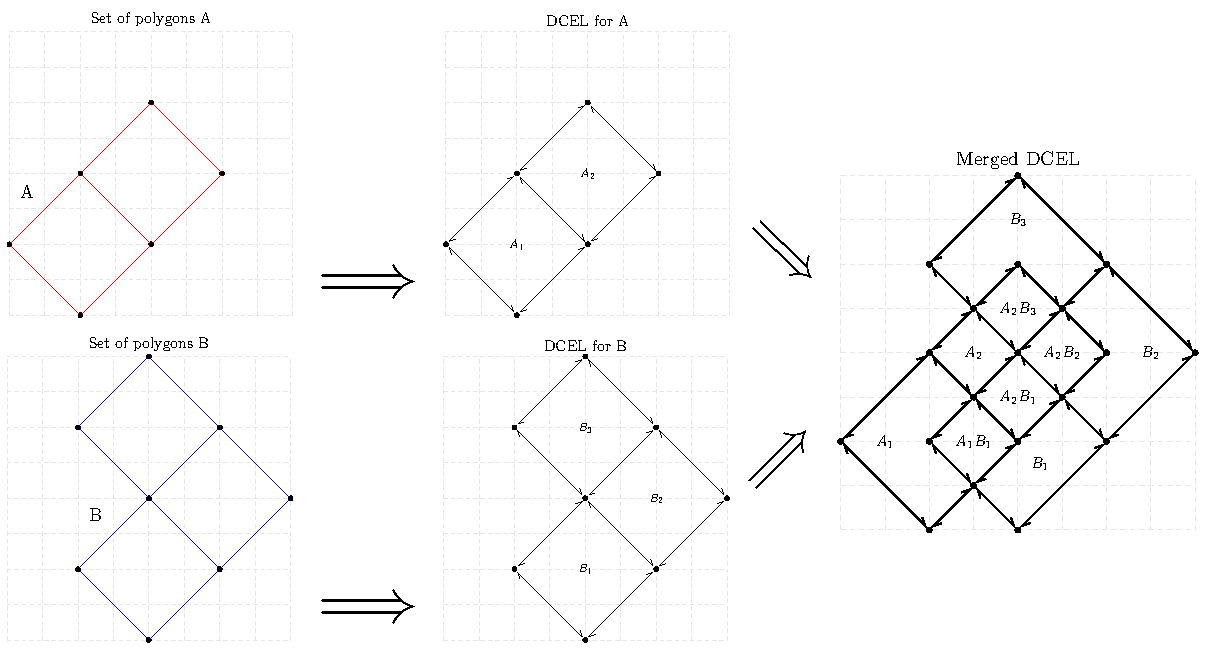
\includegraphics[width=1\linewidth]{figures/Overlay} 
\end{frame}

\begin{frame}{Overlay operation outline}
    \centering 
    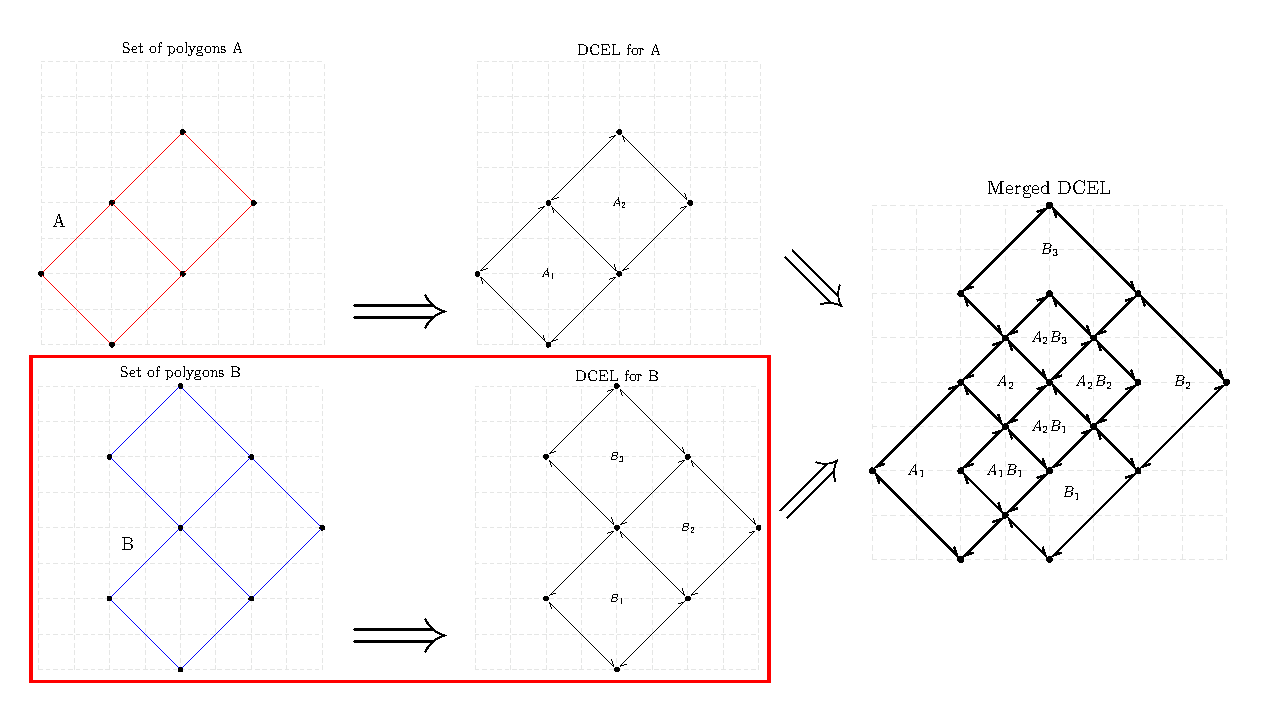
\includegraphics[width=1\linewidth]{figures/OverlayFocus} 
\end{frame}

\section{Parallel DCEL construction}
\begin{frame}{Records in the DCEL construction}
    \begin{itemize}
        \item Vertex(x: Double, y: Double, edge: Half-edge)
        \item Half-edge(origen: Vertex, twin: Half-edge, next: Half-edge, prev: Half-edge, face: Face)
        \item Face(egde: Half-edge, label: String)
    \end{itemize}
\end{frame}

\begin{frame}{DCEL construction outline}
    \begin{itemize}
        \item Input: Set of polygons.
        \item Output: Dataset of Half-edge records
        \begin{enumerate}
         \item Read set of polygons
         \item Partition set of polygons according to a grid
         \item For each partition extract its MBR polygon and clip the polygons inside each partition
         \item At each partition built the corresponding DCEL:
            \begin{enumerate}
             \item There are two approaches described in [1] and [2].  First one is done, currently working on the second one.
            \end{enumerate}
        \item Merge half-edges from each partition
        \end{enumerate}
    \end{itemize}
    
    \blfootnote{[1] \url{https://tinyurl.com/y58xk82e}}
    \blfootnote{[2] \url{https://tinyurl.com/yxnlr5uf}}
\end{frame}

\section{Example}
\begin{frame}{DCEL construction example}
    \centering 
    Set of polygons \\
    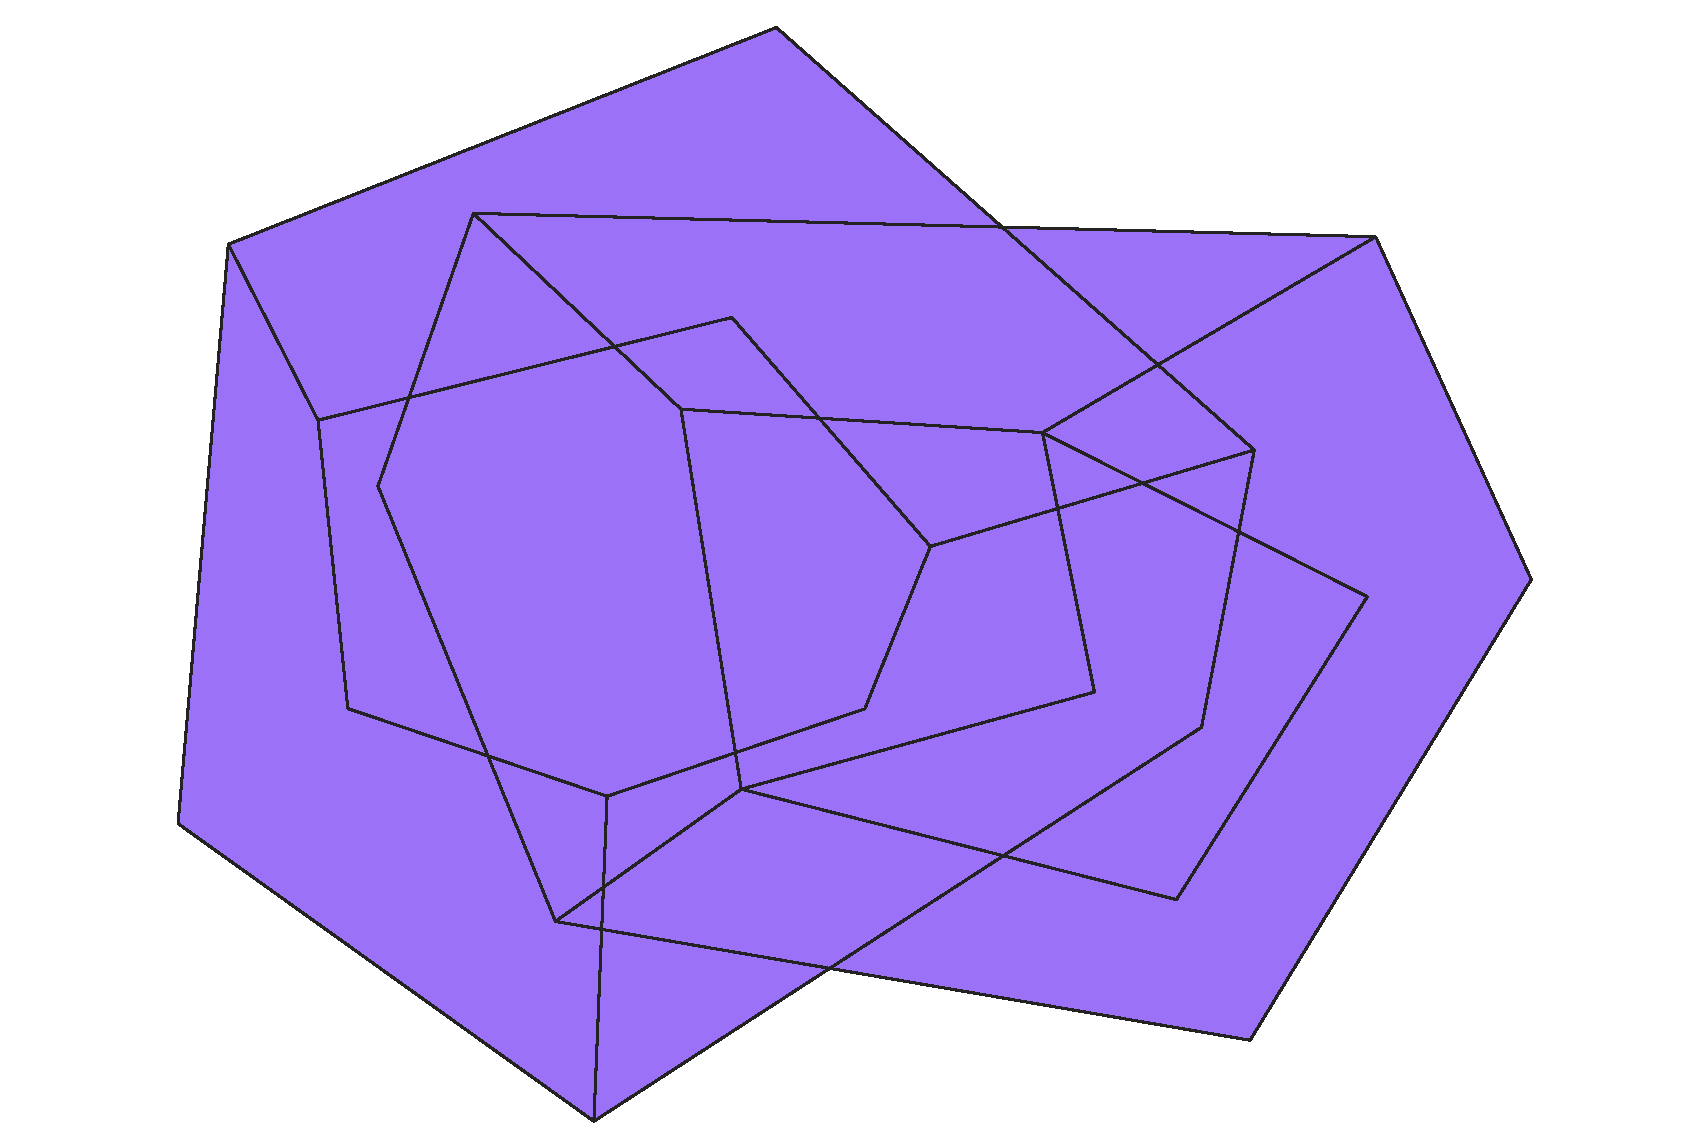
\includegraphics[width=0.8\linewidth]{figures/DCEL01_input} 
\end{frame}

\begin{frame}{DCEL construction example}
    \centering 
    Partitioning \\
    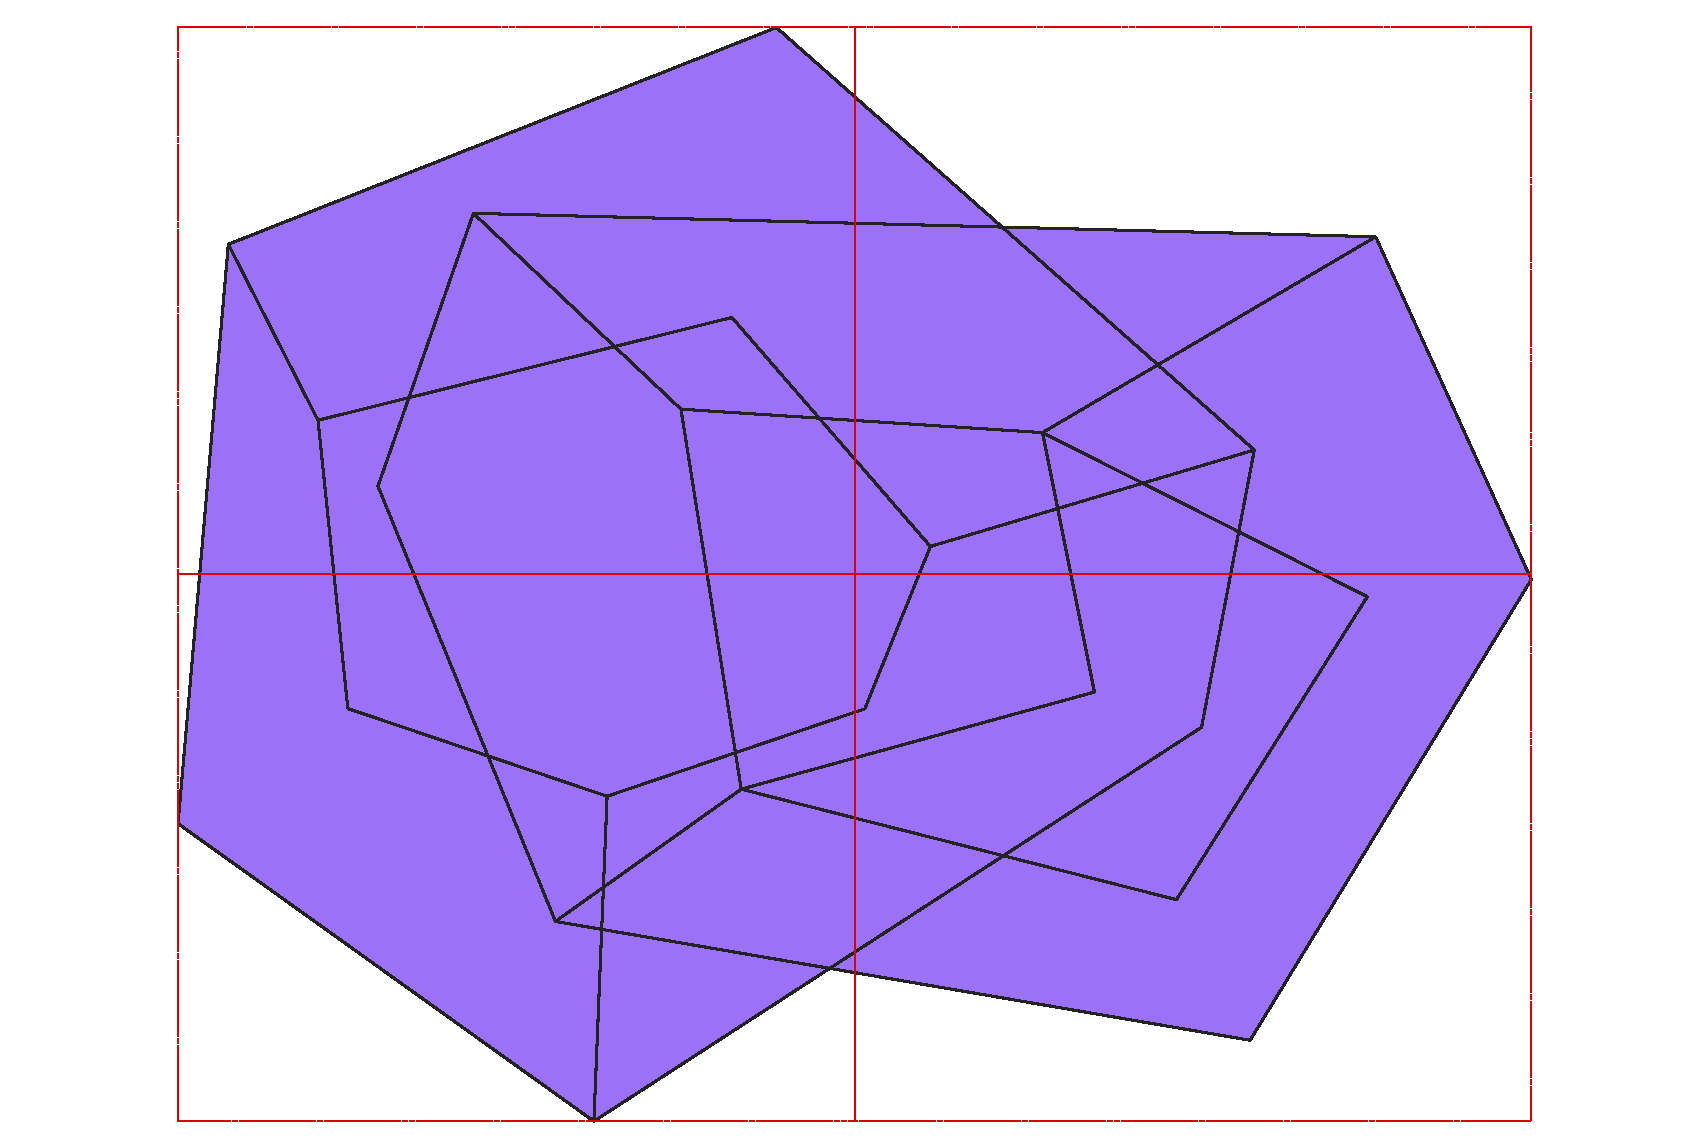
\includegraphics[width=0.8\linewidth]{figures/DCEL02_partitions} 
\end{frame}

\begin{frame}{DCEL construction example}
    \centering 
    Clipping \\
    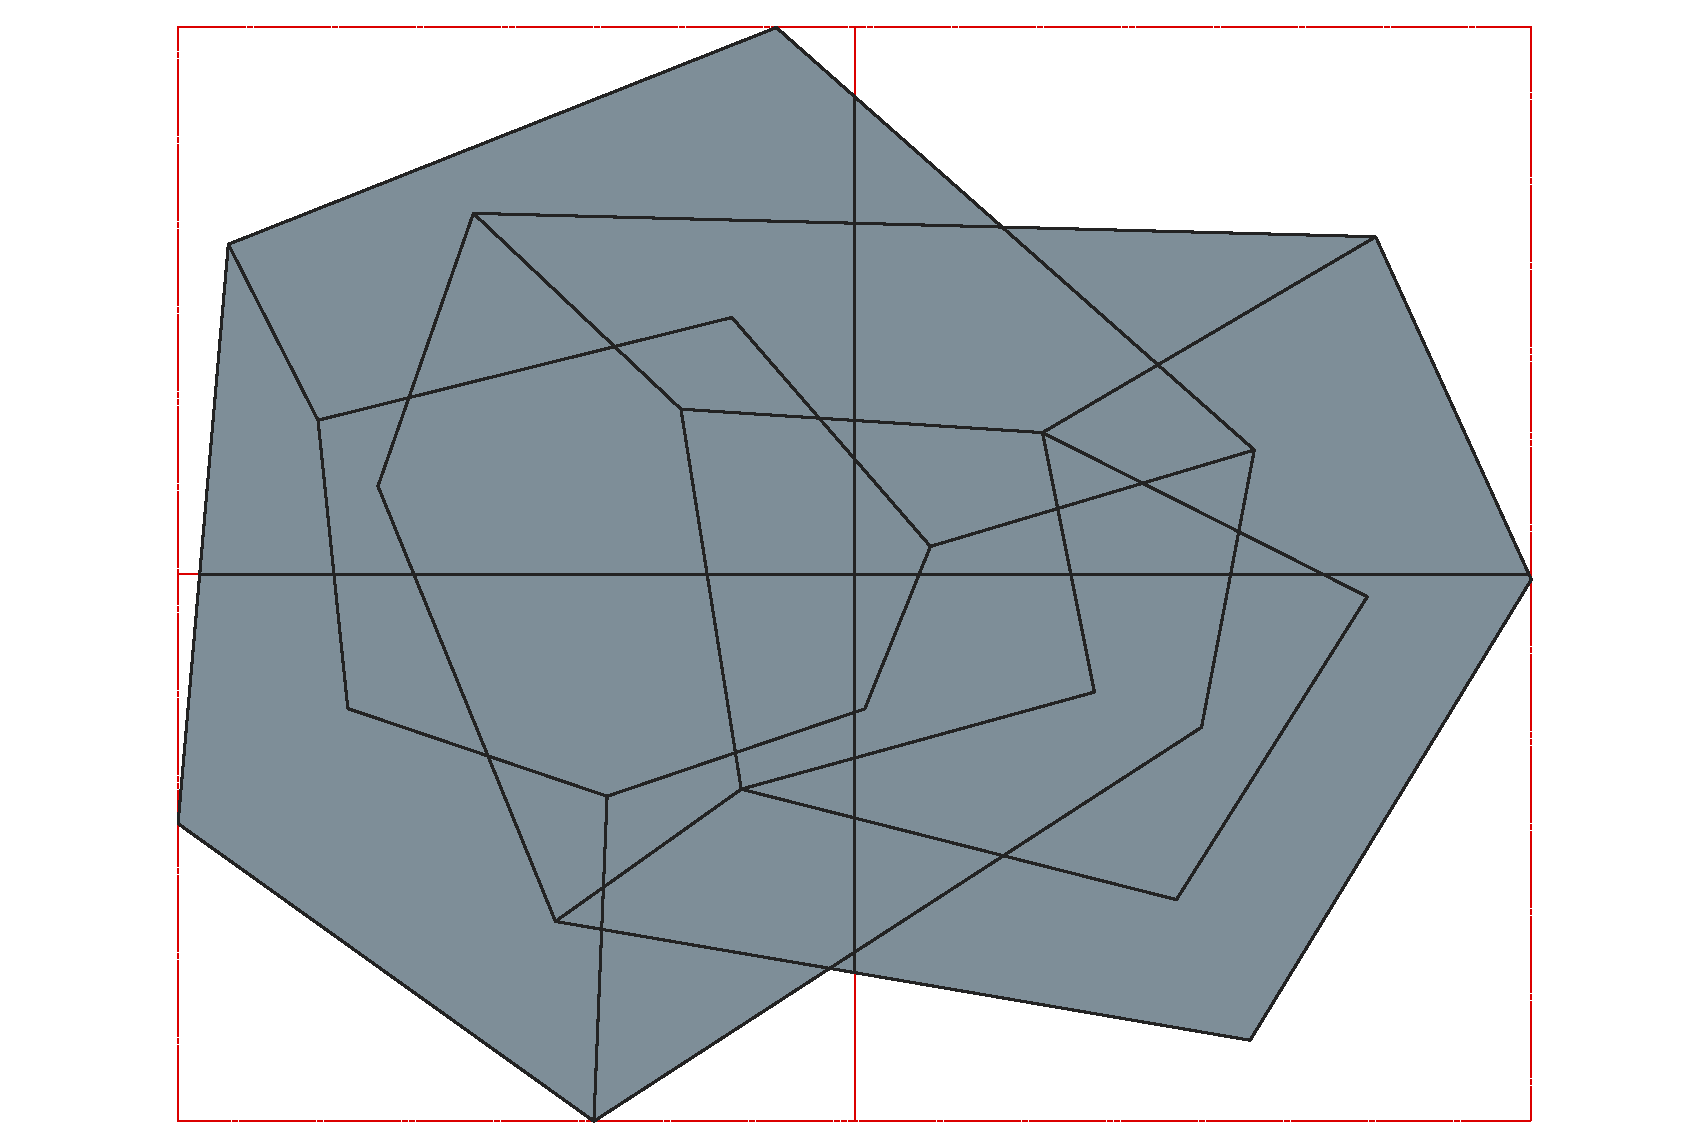
\includegraphics[width=0.8\linewidth]{figures/DCEL03_clipByPartition} 
\end{frame}

\begin{frame}{DCEL construction example}
    \centering 
    Local step input (set of clipped polygons) \\
    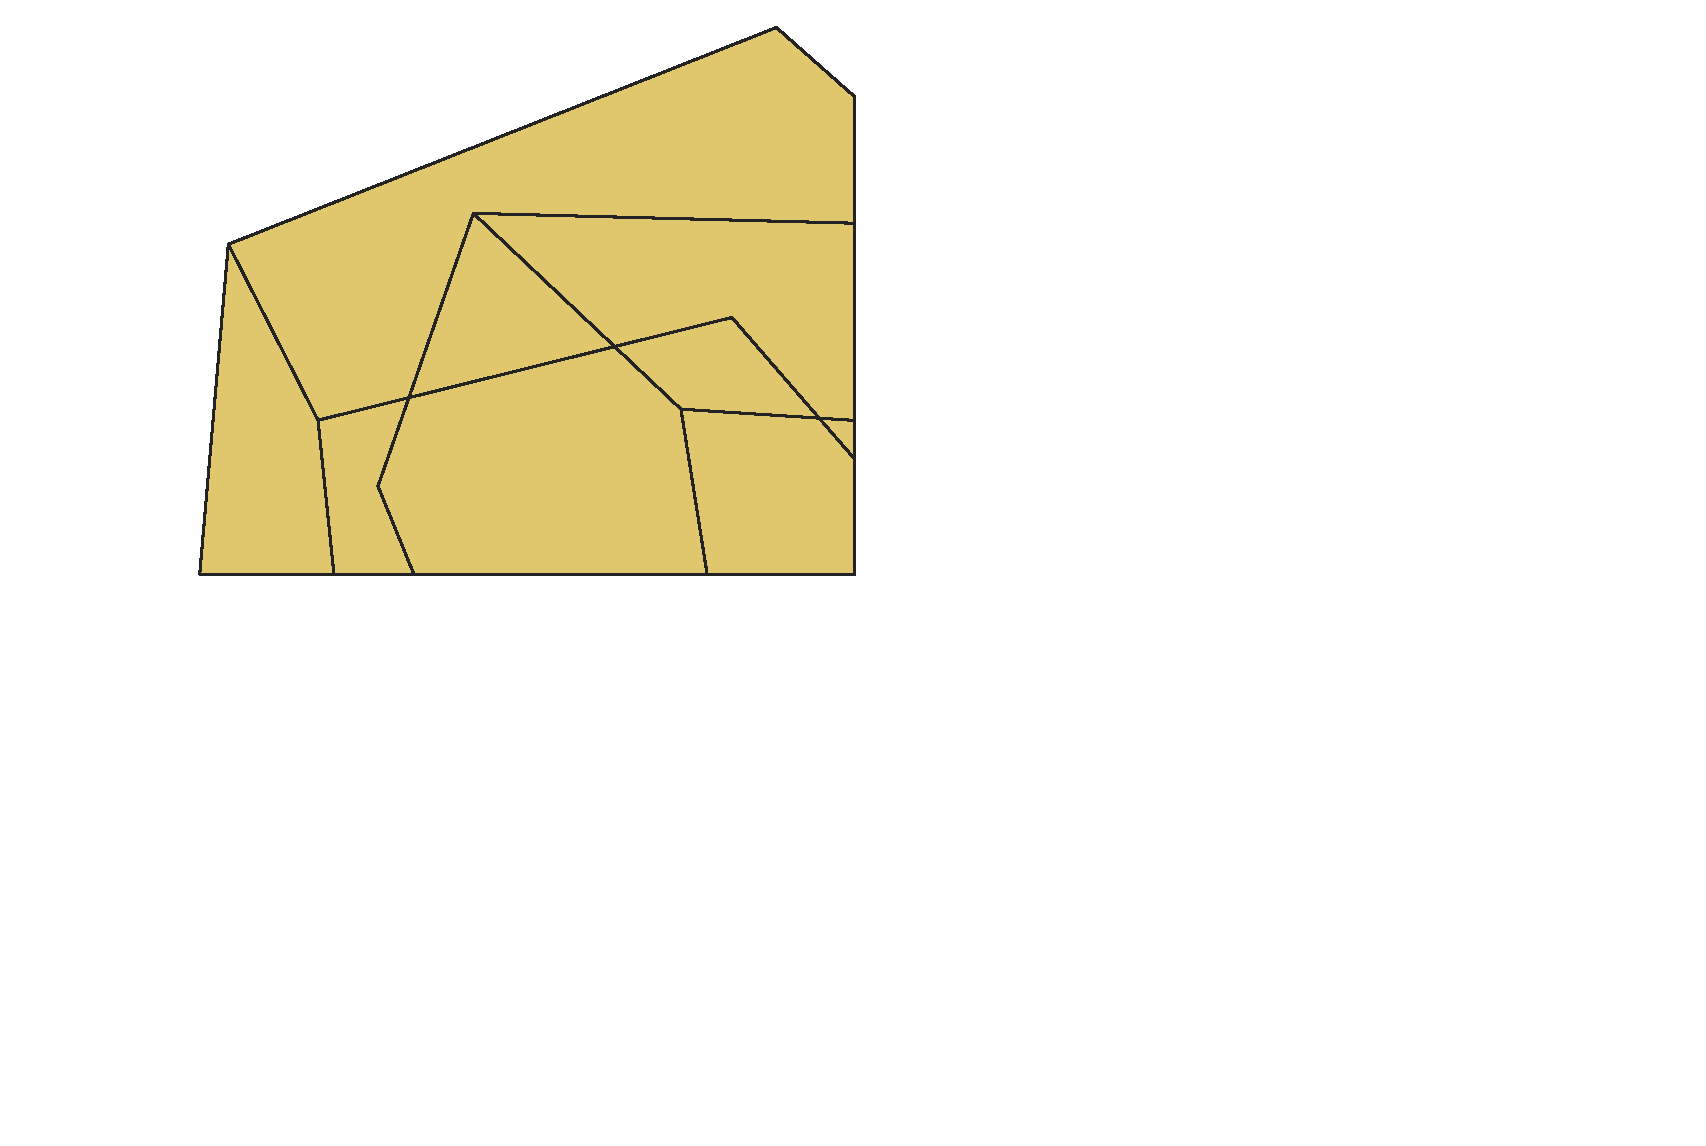
\includegraphics[width=0.8\linewidth]{figures/DCEL04_mapPartition} 
\end{frame}

\begin{frame}{DCEL construction example}
    \centering 
    Local step output (local DCEL) \\
    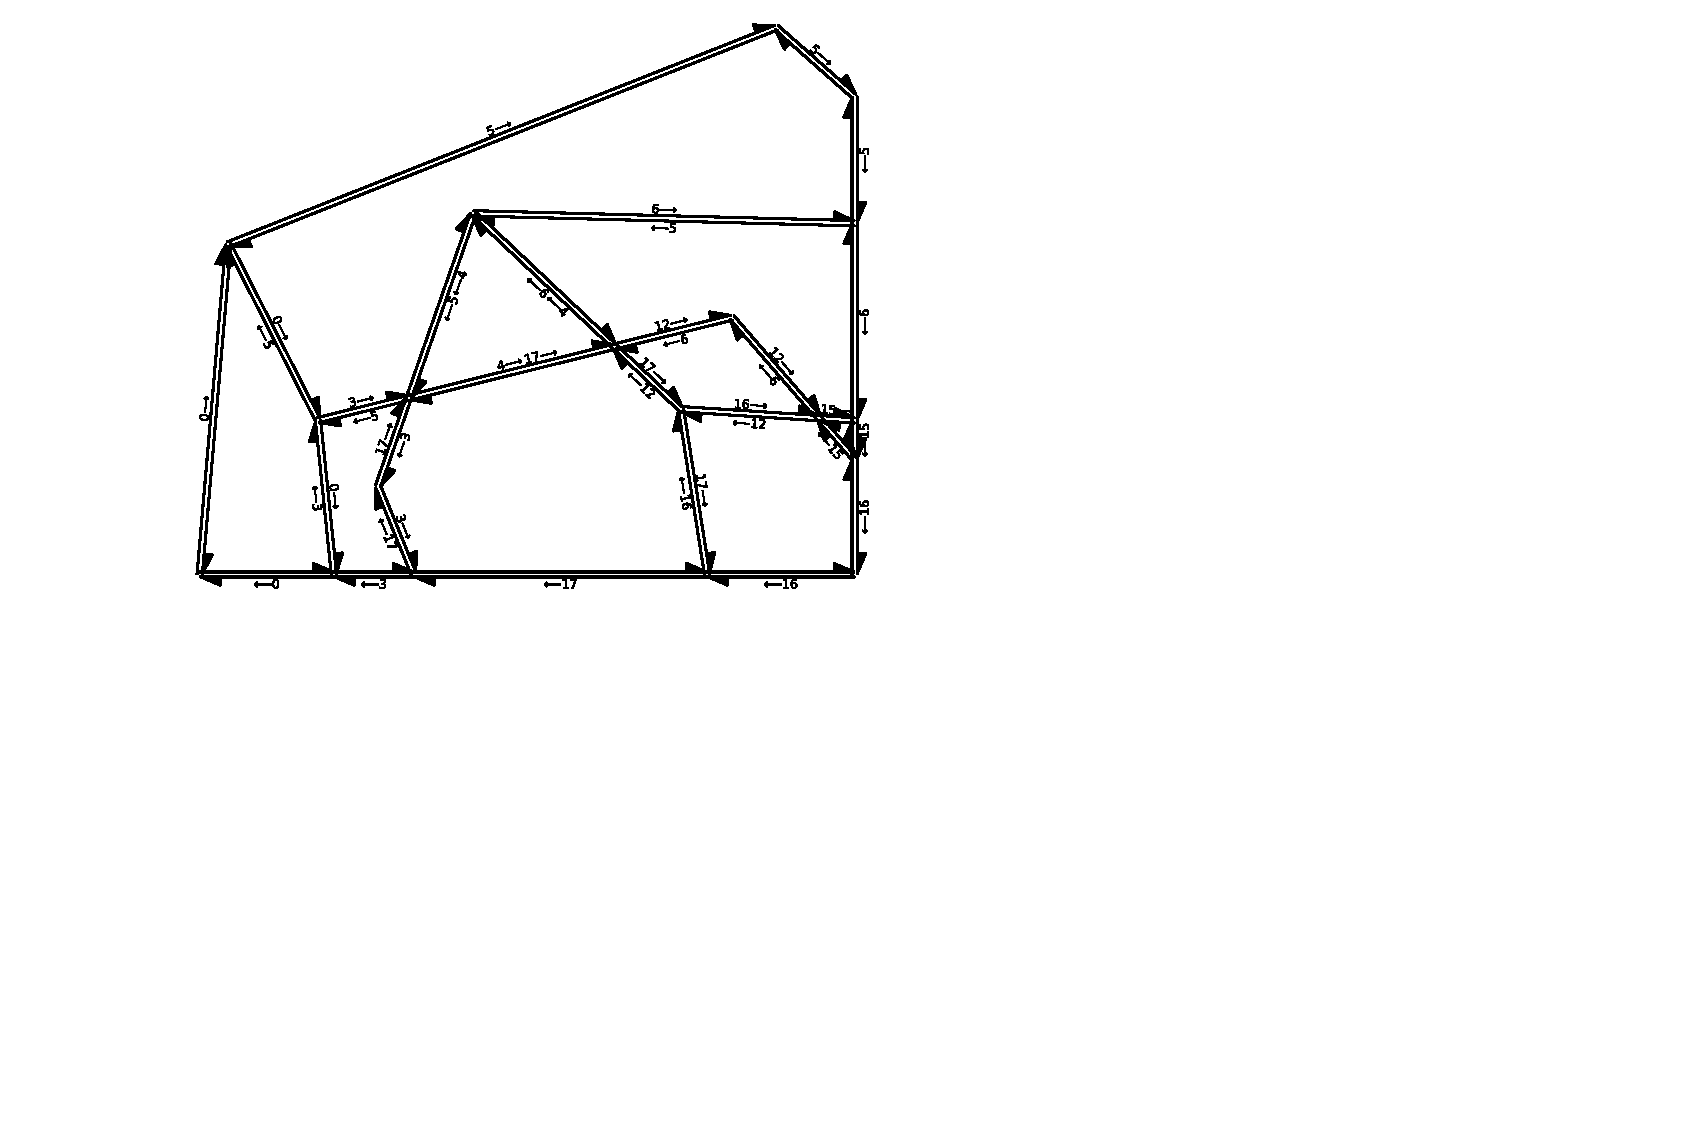
\includegraphics[width=0.8\linewidth]{figures/DCEL05_localDCEL} 
\end{frame}

\begin{frame}{DCEL construction example}
    \centering 
    Global view (DCELs at each partitions) \\
    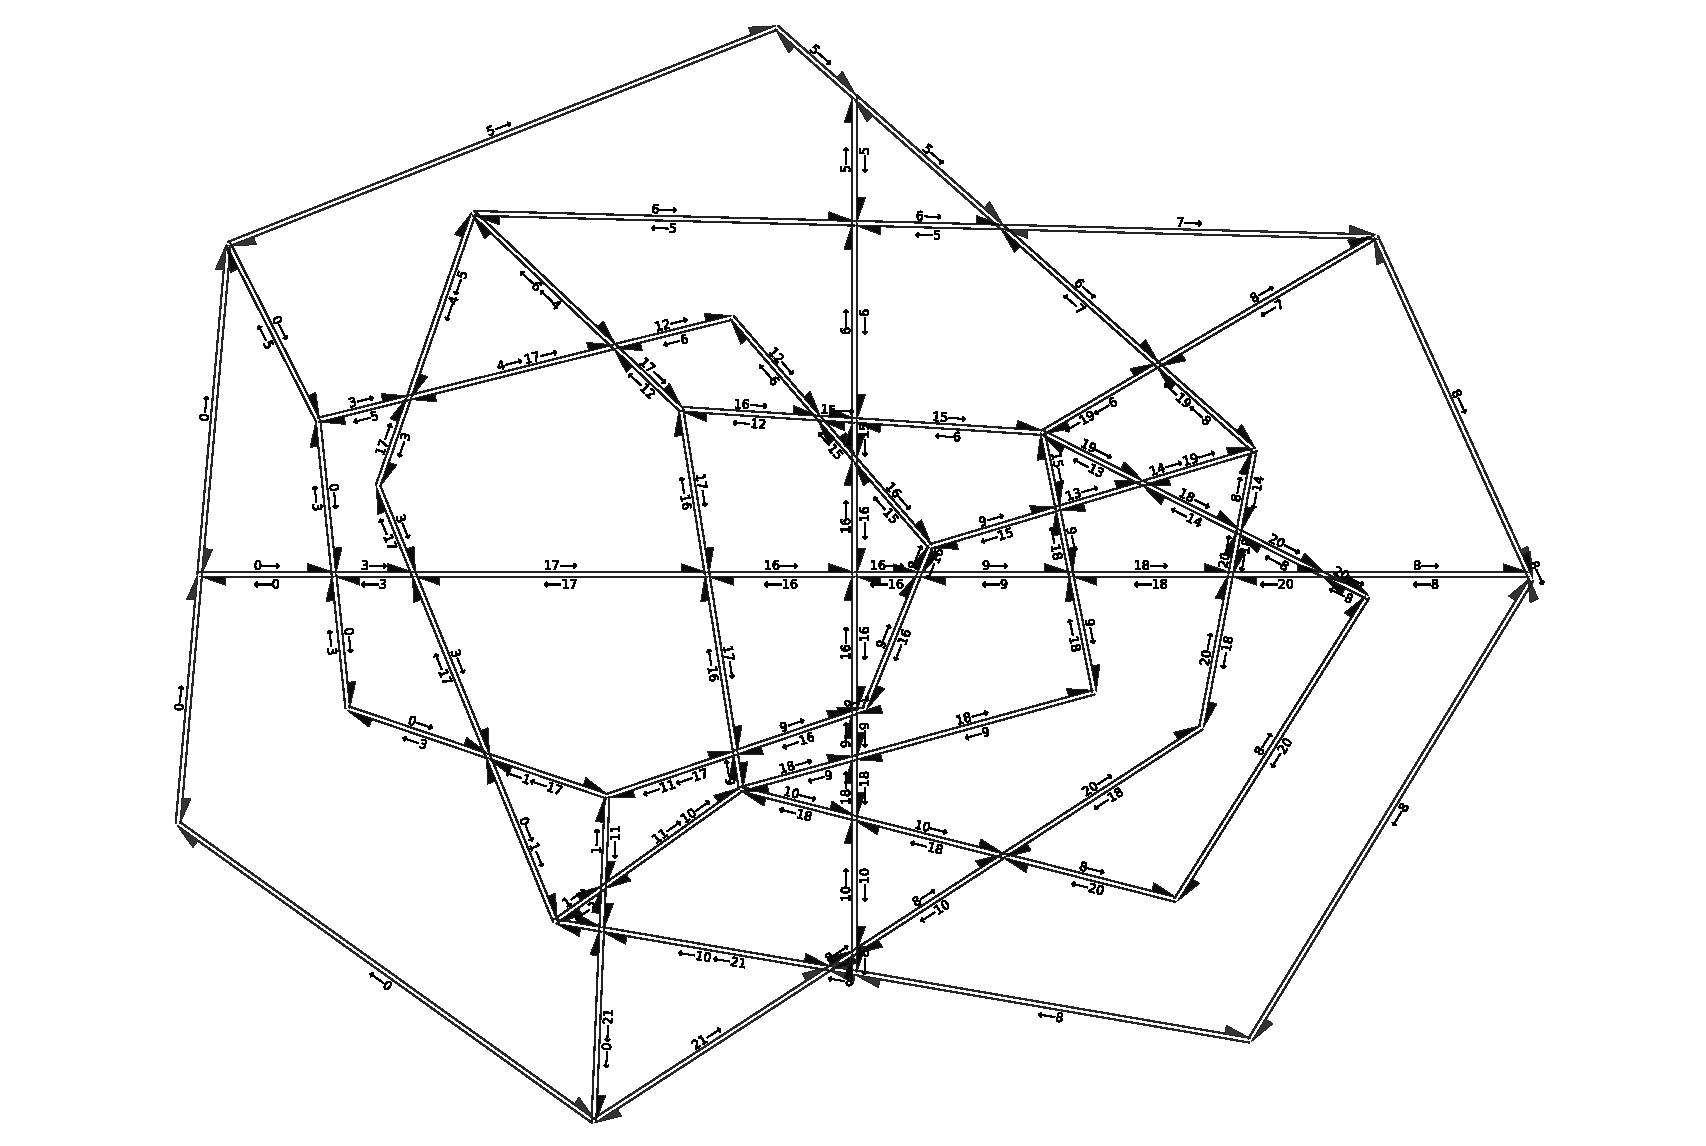
\includegraphics[width=0.8\linewidth]{figures/DCEL06_Merge} 
\end{frame}

\section{What is next}
\begin{frame}{Merged Partitioned DCEL}
    \centering 
    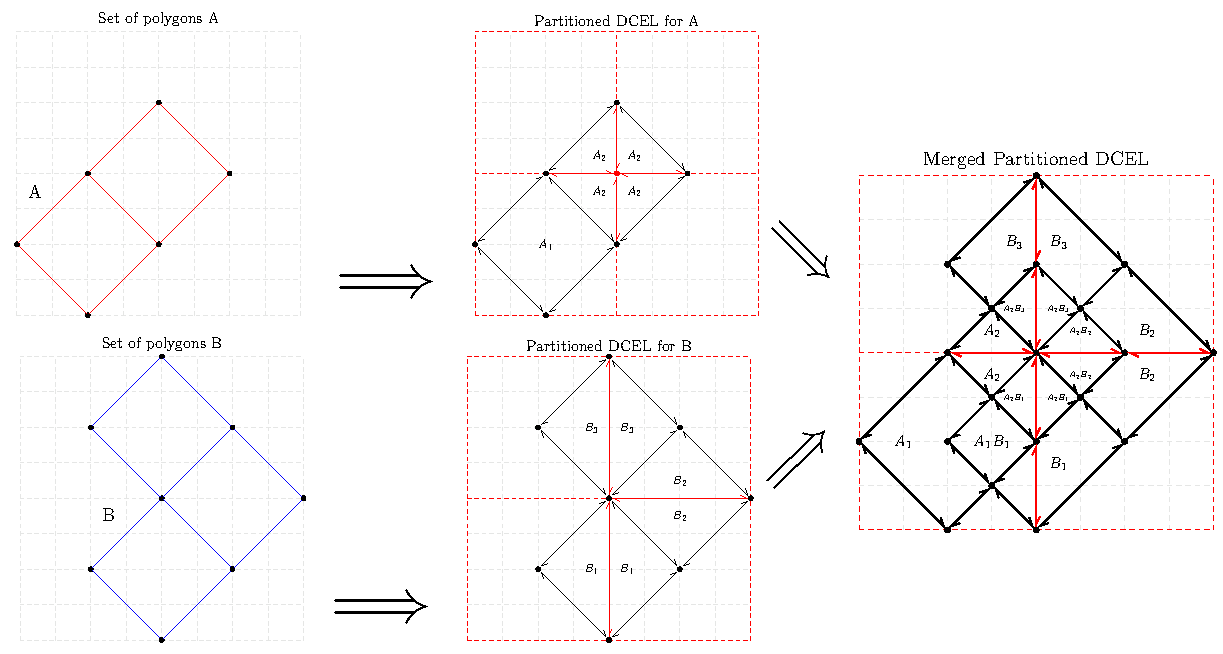
\includegraphics[width=\linewidth]{figures/OverlayParted} 
\end{frame}

\begin{frame}{Partitioned Overlay Operation}
    \centering 
    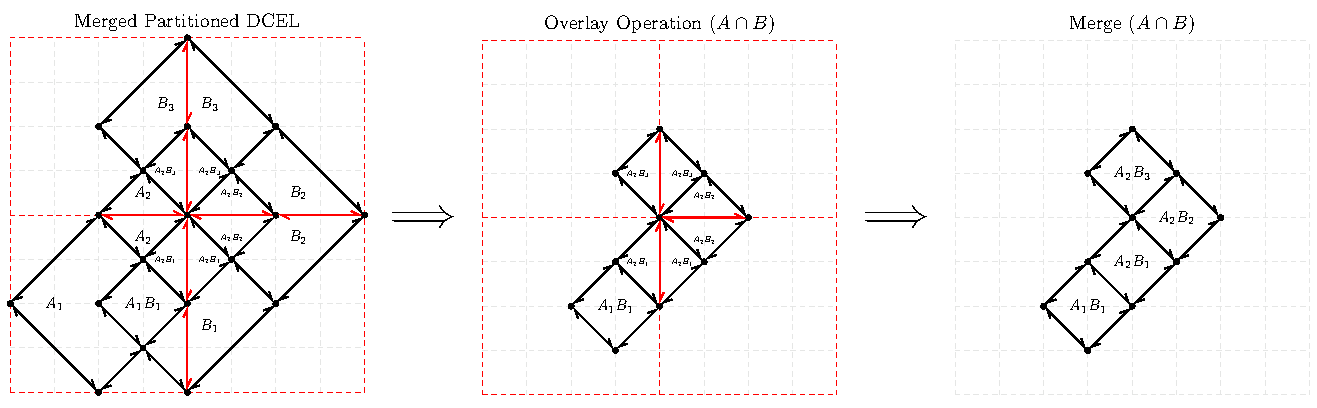
\includegraphics[width=\linewidth]{figures/OverlayParted2} 
\end{frame}

\end{document}
